
\section{Appendix}
\begin{frame}{The Max Planck Institute - Grand Ensemble \cite{maher_max_2019}}

  \begin{columns}
    \begin{column}{0.5\textwidth}
      \textcolor{purple}{\large \textbf{Field Types}}
      \begin{itemize}
        \item 32 different fields for the atmosphere
        \item Resolution: Lat/Long: $1.875 °$ , Time: monthly averages, Vertical: 26 Levels from 10 to 100000 $Pa$ 
        \item Examples: evaporation, preciptation, horizontal wind speed, specific humidity   
      \end{itemize}
      
      
    \end{column}
    \begin{column}{0.5\textwidth}

     \begin{forest}
      for tree={
        font=\ttfamily,
        grow'=0,
        child anchor=west,
        parent anchor=south,
        anchor=west,
        calign=first,
        edge path={
          \noexpand\path [draw, \forestoption{edge}]
          (!u.south west) +(7.5pt,0) |- node[fill,inner sep=1.25pt] {} (.child anchor)\forestoption{edge label};
        },
        before typesetting nodes={
          if n=1
            {insert before={[,phantom]}}
            {}
        },
        fit=band,
        before computing xy={l=15pt},
      }
    [MPI-GE
    [ \textcolor{red}{\$RCP-SENARIO}  
    [\textcolor{teal}{\$SIMULATION-TYPE}
        [\textcolor{purple}{\$FIELD-TYPE}
        [\textcolor{blue}{\$MEMBER}
              [\$VERSION
                [field.nc]
              ]
            ]
          ]
        ]
      ]
      [\textcolor{red}{historical}]
    ]
    \end{forest}     
      
    \end{column}
    
  \end{columns}
  
\end{frame}
\begin{frame}{Integrated Water Vapor Transport}

 \begin{columns}
   \begin{column}{0.5\textwidth}
    \begin{figure}[t]
      \centering
      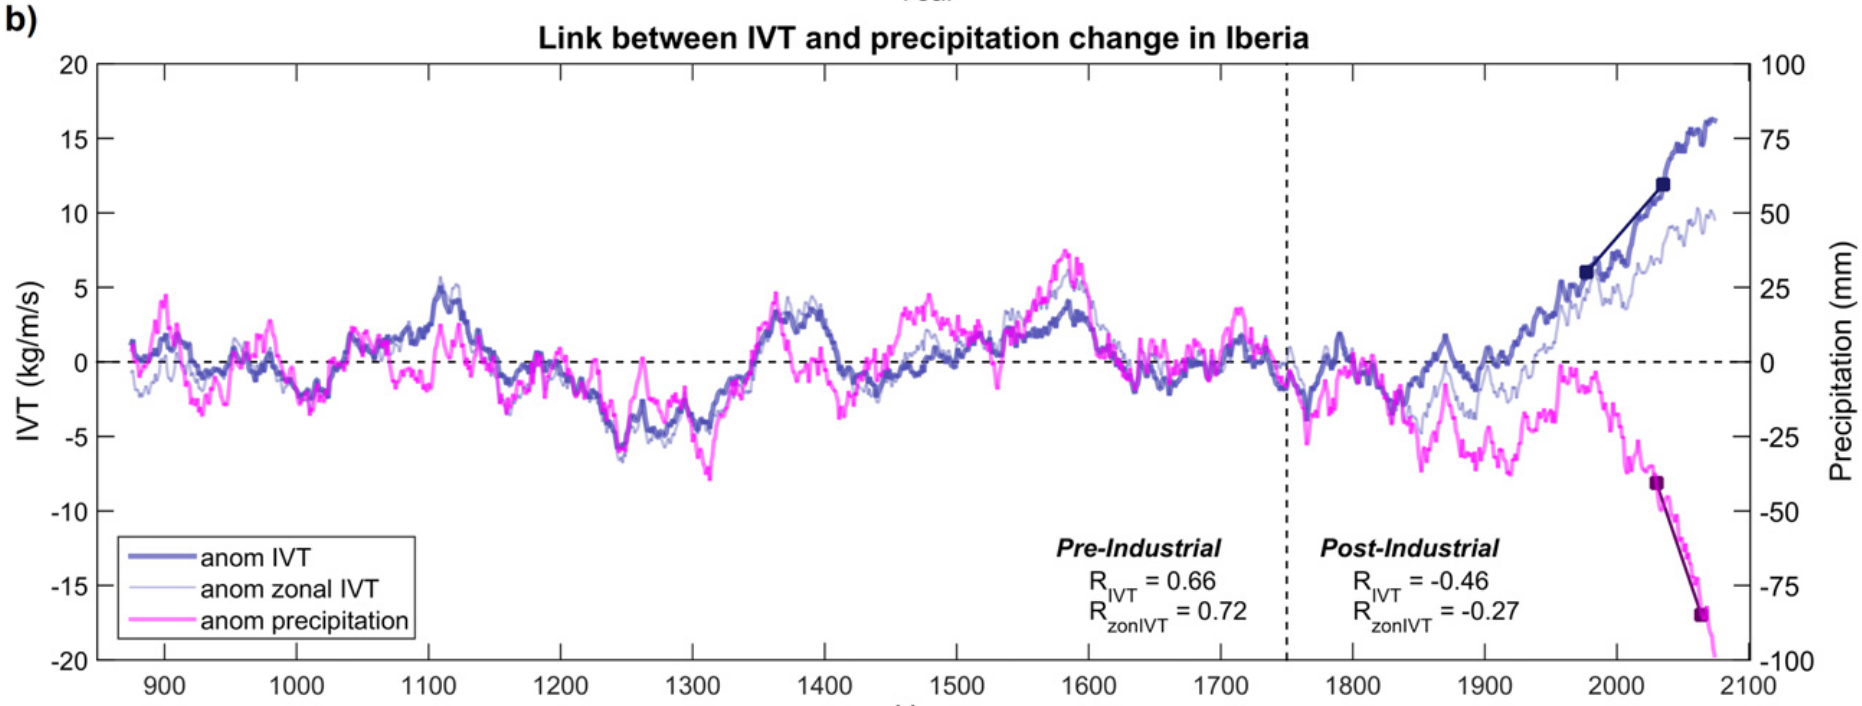
\includegraphics[width=\columnwidth]{imglib/precipitation_iberian_future.png}
    \end{figure}
    
   \end{column}
   \begin{column}{0.5\textwidth}
    \begin{figure}[t]
      \centering
      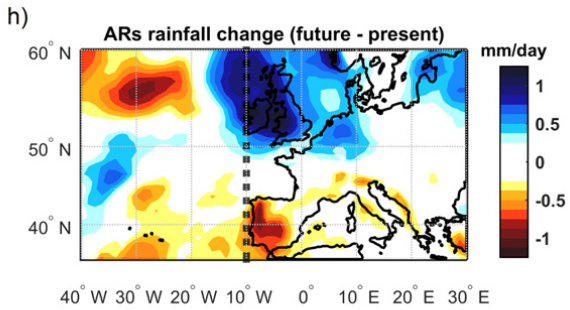
\includegraphics[width=\columnwidth]{imglib/ar_rainfall_change.png}
    \end{figure}
    
   \end{column}
  
 \end{columns} 
\end{frame}
\begin{frame}{My current plan}
  
  {\large
  \begin{enumerate}
    \item Filter the MPI-GE for my needs
    \item Generate an IVT field from the MPI-GE
    \item Implement a similar windowed EOF approach as in \cite{vietinghoff_visual_2021} to track changes in moisture transport patterns
      \begin{itemize}
        \item maybe apply concept of atmospheric rivers to the analysis
        \item maybe also implement/use some other analyses from similar work 
      \end{itemize}
    \item Visualize the uncertain Scalar Fields over time
%      \begin{itemize}
%        \item some more open questions 
%      \end{itemize}
  \end{enumerate}
}
\end{frame}


\begin{frame}{Moisture Budgets}


$$
\frac{1}{g} \frac{\delta}{\delta t} \int^{P_s}_0 q dp = - \nabla \cdot \frac{1}{g} \int^{P_s}_0 (qv) dp + E - P
$$
  
\end{frame}
